\chapter{Sistemas de Gestão de Aprendizado}
\thispagestyle{empty} % retira numeracao da pagina, conforme as normas de apresentacao.

Um sistema de gestão de aprendizagem (SGA/LMS), também chamado de um ambiente virtual de aprendizagem (AVA), é um software que permite a criação de cursos na forma de sistemas on-line \cite{article:sclater}. Um LMS é geralmente um sistema protegido mediante autenticação e autorização de recursos que permite que a instituição de ensino disponibilize vários ambientes de cursos com relativa facilidade. O ambiente do curso é normalmente gerido pelo instrutor (educador). O educador tem a autorização para fazer \textit{upload} de conteúdo para o \textit{site}, organizar os materiais no continuum educativo que reflete o curso, grupos de discussão abertos e gerenciar as informações enviadas para os grupos de notícias, incluindo a moderação de conteúdos impróprios. O educador pode visualizar relatórios dos usuários, receber atividades e trabalhos dos alunos, a fim de avaliá-lo. Em muitos LMSs o sistema está ligado a outros sistemas administrativos na organização, tais como o sistema de matrícula, o sistema de lançamento de notas, e assim sucessivamente. As permissões dos alunos são geralmente mais limitadas do que as do educador. Alunos inscritos em um determinado curso podem visualizar o conteúdo e baixá-lo. Eles podem participar de atividades interativas que acontecem em fóruns e em alguns casos também podem contribuir com conteúdo em locais específicos, tais como ambientes wiki ou repositórios especiais de colaboração definidos pelo gestor do curso. Diferentes sistemas de gestão de aprendizagem têm diferentes interfaces de usuário e características diferentes. No entanto, todos eles compartilham três funções-chave \cite{website:morgan} \cite{article:coats-baldwin}.

\begin{itemize}
    \item Sistema de gerenciamento de conteúdo: Permite  a criação ou o \textit{upload} de uma variedade de itens de conteúdo, como textos, apresentações, artigos digitalizados e materiais audio-visual. O sistema de gerenciamento de conteúdo também permite que o material a ser organizado em uma estrutura planejada pelo administrador do curso, criando pastas para temas e conteúdos.
    \item Ferramentas para gerenciamento de interações: Diferentes sistemas de gestão de aprendizagem permitem que o instrutor para abrir diferentes fóruns. Alguns sistemas permitem a abertura de espaços assíncronos de colaboração, tais como \textit{wikis} e \textit{blogs}, e alguns podem fornecer comunicação síncrona usando bate-papo e outras ferramentas de conferência \textit{on-line}.
    \item Ferramentas para gerenciar e avaliar alunos: Alguns sistemas fornecem ferramentas administrativas para tarefas de gravação, notas e \textit{feedback}. Eles também fornecem relatórios de usuários que suportam o instrutor na medição do nível da participação dos alunos e na avaliação das realizações dos alunos.
\end{itemize}


\section{Requisitos principais dos SGAs}

De acordo com Scott \cite{article:scott}, os requisitos funcionais de um LMS mais comuns nas plataformas existentes, são apresentados na tabela \ref{funcs_comuns}.

No entanto, pode-se observar uma discrepância na ordem em que aparecem as funcionalidades quando considerada a importância da funcionalidade na tomada de decisões de escolha da ferramenta de ensino, como visto na tabela \ref{funcs_importantes}.

Além disso, é importante ressaltar que estudos recentes concluíram que poucos usuários utilizam das funcionalidades mais avançadas e apresentam maior satisfação ao utilizar as funcionalidades consideradas mais básicas \cite{report:educause}.
Outro grande fator considerado neste trabalho, é a demanda existente do acesso ao LMS em dispositivos móveis entre os usuários \cite{report:educause}.

\begin{table}[H]
\centering
\caption{Funcionalidade mais comuns em SGAs}
\begin{tabular}{lll}
Funcionalidade & \begin{tabular}[c]{@{}l@{}}Número de produtos \\ que possuem\\ a funcionalidade\end{tabular} & \begin{tabular}[c]{@{}l@{}}Percentual do total (45) \\ de produtos que possuem\\ a funcionalidade\end{tabular} \\
Forums de discussão & 41 & 91.11\% \\
Matrícula no curso/disciplina & 41 & 91.11\% \\
Mensagens/Notificações Internas & 39 & 86.67\% \\
Autenticação & 38 & 84.44\% \\
Bate-papo & 34 & 75.56\% \\
Ajuda/Suporte & 34 & 75.56\% \\
Trabalho em grupo & 34 & 75.56\% \\
Auto-avaliação & 34 & 75.56\% \\
Moderação de conteúdo & 34 & 75.56\% \\
Exames e notas & 34 & 75.56\% \\
Disponibilização de Arquivos & 33 & 73.33\% \\
Datas/Eventos Importantes & 33 & 73.33\%
\end{tabular}
\label{funcs_comuns}
\end{table}



\begin{table}[H]
\centering
\caption{Funcionalidade mais importantes em SGAs}
\label{funcs_importantes}
\begin{tabular}{lll}
Funcionalidade & \begin{tabular}[c]{@{}l@{}}Número de vezes que funcionalidade\\ influenciou a escolha\end{tabular} & \begin{tabular}[c]{@{}l@{}}Percentual\\ (de 1720 total de decisões)\end{tabular} \\
Fórums de Discussão & 1076 & 62.56 \\
Gerenciamento de Curso & 866 & 50.35 \\
Disponibilização de Arquivos & 818 & 47.56 \\
Acompanhamento de Aluno & 802 & 46.63 \\
Exames e Notas & 751 & 43.66 \\
Lançamento de Notas & 743 & 43.2 \\
Mensagens/Notificações Internas & 741 & 43.08 \\
Trabalho em Grupo & 740 & 43.02 \\
Bate-papo & 730 & 42.44 \\
Auto avaliação & 712 & 41.4 \\
Modelos de Cursos & 692 & 40.23 \\
Autenticação & 687 & 39.94
\end{tabular}
\end{table}




Dessa forma, são contempladas no escopo do projeto proposto apenas as funcionalidades expositivas mais comuns e consideradas mais importantes para sistemas deste tipo. O enfoque da aplicação se dará em notificar e apresentar para os alunos inscritos nos cursos os conteúdos disponibilizados e comunicações disseminadas através das plataformas registradas no aplicativo, de modo que estas informações possam ser agregadas de forma homogênea e transparente no que se refere a origem daquela informação.



\section{SGAs Referenciais}

Os fatores determinantes para a escolha dos SGA nos quais este projeto se baseia, na forma como a arquitetura do software foi projetada e de que forma se permitirá sua extensibilidade, foram os seguintes:
\begin{itemize}
    \item Presença das funcionalidades comuns mais importantes
    \item Tipo e custo de licença de uso do software
    \item Capacidade e facilidade de extensão do software
    \item Adesão e familiaridade no uso da ferramenta já existente na comunidade acadêmica da instituição onde se encontra o público alvo
    \item A existência de uma camada de serviço que possibilite o acesso dos recursos do software através da rede móvel do usuário 
\end{itemize}

No que se refere as funcionalidades disponíveis nos SGAs existentes, fizemos o seguinte levantamento com as ferramentas líderes de mercado e aquela disponibilizada oficialmente e desenvolvida pela instituição onde se encontra o público alvo do projeto. Os resultados podem se observar na tabela \ref{funcs_sga}.

\begin{table}[H]
\centering
\caption{Funcionalidades disponíveis por SGAs}
\label{funcs_sga}
\begin{tabular}{@{}llll@{}}
\toprule
Funcionalidade & Blackboard & Moodle & Conexão UFF \\ \midrule
Fórums de Discussão & sim & sim & sim \\
Notificações/Mensagens Internas & sim & sim & sim \\
Disponibilização de Arquivos & sim & sim & sim \\
Integração com Sistema de Matrícula & possível & possível & sim \\
Exames e Notas & sim & sim & não \\
Integração com Lançamento de Notas & possível & possível & possível \\
Mensagens/Notificações Internas & sim & sim & sim \\
Trabalho em Grupo & sim & sim & não \\
Bate-papo & sim & sim & em desenvolvimento \\
Suporte/Ajuda & sim & sim & sim \\ \bottomrule
\end{tabular}
\end{table}

Visto que as plataformas de código aberto são adequadas para as universidades e outras instituições de ensino \cite{article:itmazi}, pelos seguintes motivos: 
\begin{enumerate}
    \item Elas permitem que instituições de ensino tenham controle do software
    \item O custo de usar a licença é muito baixo ou inexistente
    \item Licença de código aberto permite qualquer alteração, modificação e melhoria no LMS.
\end{enumerate}



Desta forma, foi selecionada a rede social de fins acadêmicos disponibilizada pela Universidade Federal Fluminense, o Conexão UFF, por possuir a maior parte das funcionalidades consideradas mais comuns e mais importantes, e especialmente por já ser uma ferramenta amplamente utilizada na instituição, com adesão de mais de 57\% das disciplinas oferecidas na Universidade, para ao menos alguma funcionalidade, além de oferecer uma camada de serviços que possibilite o desenvolvimento do projeto. Também foi adotado como referencial a ferramenta \textit{open source} líder de mercado e já utilizada em alguns cursos da Universidade, o Moodle, que como visto na tabela \ref{funcs_sga} também comtempla as funcionalidades consideradas mais comuns e importantes em um LMS, além de também disponibilizar uma camada de serviços.

\subsection{Conexão UFF}

A plataforma foi inicialmente concebida como projeto pessoal de um membro da Superintendência de Tecnologia da Informação da UFF e aluno do curso de Sistemas de Informação sob o nome "Orkuff", que fazia alusão a rede social \textit{Orkut}, ainda muito popular na época.

Em 2011 a plataforma foi lançada oficialmente pela universidade sob o nome de Conexão UFF, já integrada ao sistema único de autenticação da UFF, o Iduff. Dentre as funcionalidades apresentadas na versão inicial estavam os grupos, formados por participantes das respectivas turmas das disciplinas dos cursos, com recursos de fórums de discussão, upload de arquivos e troca de mensagens diretas. O professor automaticamente recebia permissões de moderação do referido grupo.

\subsubsection{Camada de Serviços}

Para o escopo desse trabalho foi criada uma camada de serviços na aplicação do Conexão UFF de modo que os recursos disponíveis no sistema pudessem ser expostos através de uma arquiterura de serviços \textit{RESTful}.

Para cada um dos recursos disponíveis foi criado um ponto de acesso, que exibe as informações permitidas para o cliente autenticado.

A autenticação é feita pela camada de serviços do Sistema Único de Autenticação da UFF, o IDUFF. O processo de autenticação se dá através dos seguintes passos:

\begin{enumerate}
    \item O usuário cadastra suas credenciais, IDUFF e Senha, no aplicativo.
    \item O aplicativo faz uma requisição ao serviço do IDUFF enviando as credenciais salvas no aplicativo
    \item O serviço de autenticação do IDUFF valida as credenciais e caso se confirme a validade dos dados, um token de acesso é enviado ao Cliente, com validade de 20 minutos.
    \item A cada requisição às APIs do Conexão UFF, o token é enviado junto ao pedido
    \item O Conexão UFF verifica através do serviço do IDUFF se o token enviado é válido e caso se confirme a validade o IDUFF estende a validade do token por mais 20 minutos.
    \item Com o token validado o Conexão continua com o processamento do pedido e responde à requisição com o conteúdo requisitado.
\end{enumerate}

A arquitetura da camada de serviços do conexão UFF é apresentada na \ref{conexao-arq}

O formato escolhido para a transferência dos dados oriundos do Conexão UFF foi o JSON, por conta da fácil manipulação nativa dos objetos pelo Javascript, linguagem escolhida para o desenvolvimento da aplicação cliente, definido em \ref{sec:client-side}.


\begin{figure}[H]
\centering
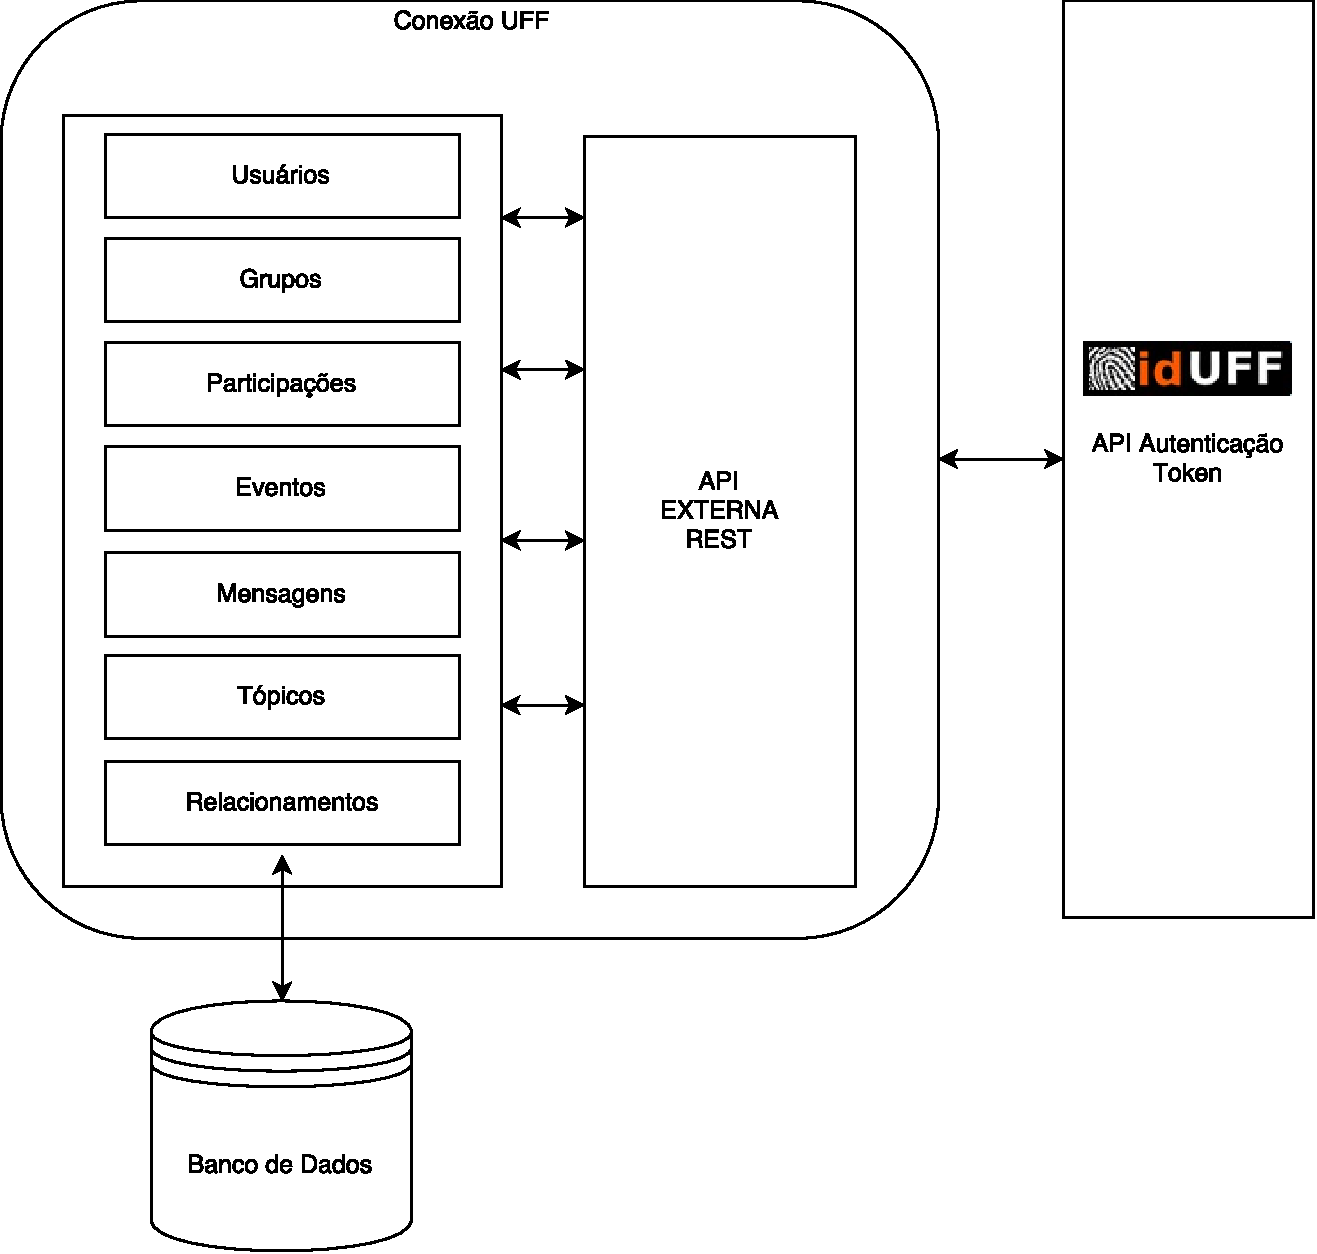
\includegraphics[scale=.65]{2_2.pdf}
    \caption{Arquitetura da camada de Serviços Conexão UFF}
    \label{conexao-arq}%
\end{figure}




\subsection{Moodle}

A plataforma mais utilizada para cursos acadêmicos on-line é o Moodle. O Moodle é um pacote de software especialmente concebido para ajudar professores a criar cursos online e oferece as funcionalidades de um LMS completo \cite{article:desnica-letic}

 O Moodle é um software de código aberto, que pode ser baixado gratuitamente a partir da Internet, usado, modificado, e até mesmo distribuído (sob uma licença GNU). O Moodle é facilmente executado em UNIX, Linux, Windows, Mac OS X, ou qualquer outro sistema que suporte PHP. Todos os seus dados são gravados em um único banco de dados, MySQL ou PostgreSQL são os mais suportados; no entanto, Oracle, Access, Interbase e ODBC  também podem ser utilizados com algumas configurações.
Dentre as funcionalidades do Moodle estão incluídos os fóruns, recursos de publicação de conteúdo, questionários, chats, atribuições, e outros recursos que geralmente são suficientes para a criação de cursos padrão. 

A unidade organizacional básica do Moodle é o curso, que é acessado através de uma página web. Um curso é organizado em seções que podem corresponder aos tópicos ou semanas, aparecendo na coluna do meio da página. É possível incluir diferentes recursos e atividades em todas as seções. O último está a ser atribuído como casa ou classe trabalho a ser desenvolvido pelos alunos. Os usuários são outro objeto Moodle essencial: eles podem se inscrever em cursos diferentes, como administradores, professores ou estudantes. Cada função é definida por suas capacidades em um determinado contexto, o que significa que eles têm um conjunto de privilégios ao executar determinadas ações \cite{article:isljamovic-petrovic}.

De acordo com o estudo realizado nos Estados Unidos \cite{article:wexler}, Blackboard e Moodle são os LMS com maior quota de mercado, sendo que o Moodle tem maior satisfação entre os usuários. Em nosso projeto, Blackboard foi descartado e escolhemos Moodle, pois além de ser \textit{Open Source}, ele já é utilizado em diversos cursos da \textit{UFF}.

\subsubsection{Camada de Serviços}
Moodle é composto por três elementos principais: o \textit{Core}, os módulos de atividades e os \textit{Plugins}. O \textit{Core} inclui as funcionalidades básicas da plataforma de aprendizagem, tais como o fórum, wiki e atividades.

Os \textit{Plugins} são blocos de software que adicionam extensões funcionais ao sistema. Dentro do Moodle, diferentes interfaces de plug-ins podem ser encontradas. Uma destas interfaces é a interface de Serviços Web, que é extensível e garante a escalabilidade do sistema em função dos diversos protocolos de comunicação.

Em 2008 foi projetada uma solução para fornecer algumas das funcionalidades através de Serviços Web, esta solução foi a Arquitetura de Serviços do Moodle, que foi implementada para Moodle 2.0 e lançada no final de 2009 \cite{article:alier}. 

A arquitetura de Serviços do Moodle acrescenta duas camadas lógicas à arquitetura do Moodle (mostrado na Figura \ref{moodle-arq}). A primeira é API externa, um conjunto de arquivos php que incluem a lógica de cada serviço. A segunda é a camada de conectores. A arquitetura de Serviços do Moodle não está vinculada a um protocolo de webservices específica; ele é projetada para ser independente de protocolo. Para cada protocolo suportado (SOAP, REST, XML-RPC, etc.) há um módulo conector específico nesta camada. Cada conector implementa a tradução dos métodos implementados na API externa com o protocolo e sintaxe específica. Além disso, o conector também oferece outros serviços necessários como autenticação, autorização e outros serviços de infra-estrutura. A camada de conectores é uma camada expansível que permite que o adição de novos protocolos de comunicação.

Um elemento-chave na concepção da arquitetura de Serviços do Moodle é sua capacidade de ampliação baseada em plugins. A API externa pode ser estendida de forma segura, dando total controle e segurança para o administrador da plataforma. Se for necessário um novo tipo de protocolo de serviços web ou método de autenticação, um desenvolvedor pode criar um novo conector de webservices para implementá-lo.

\begin{figure}[H]
\centering
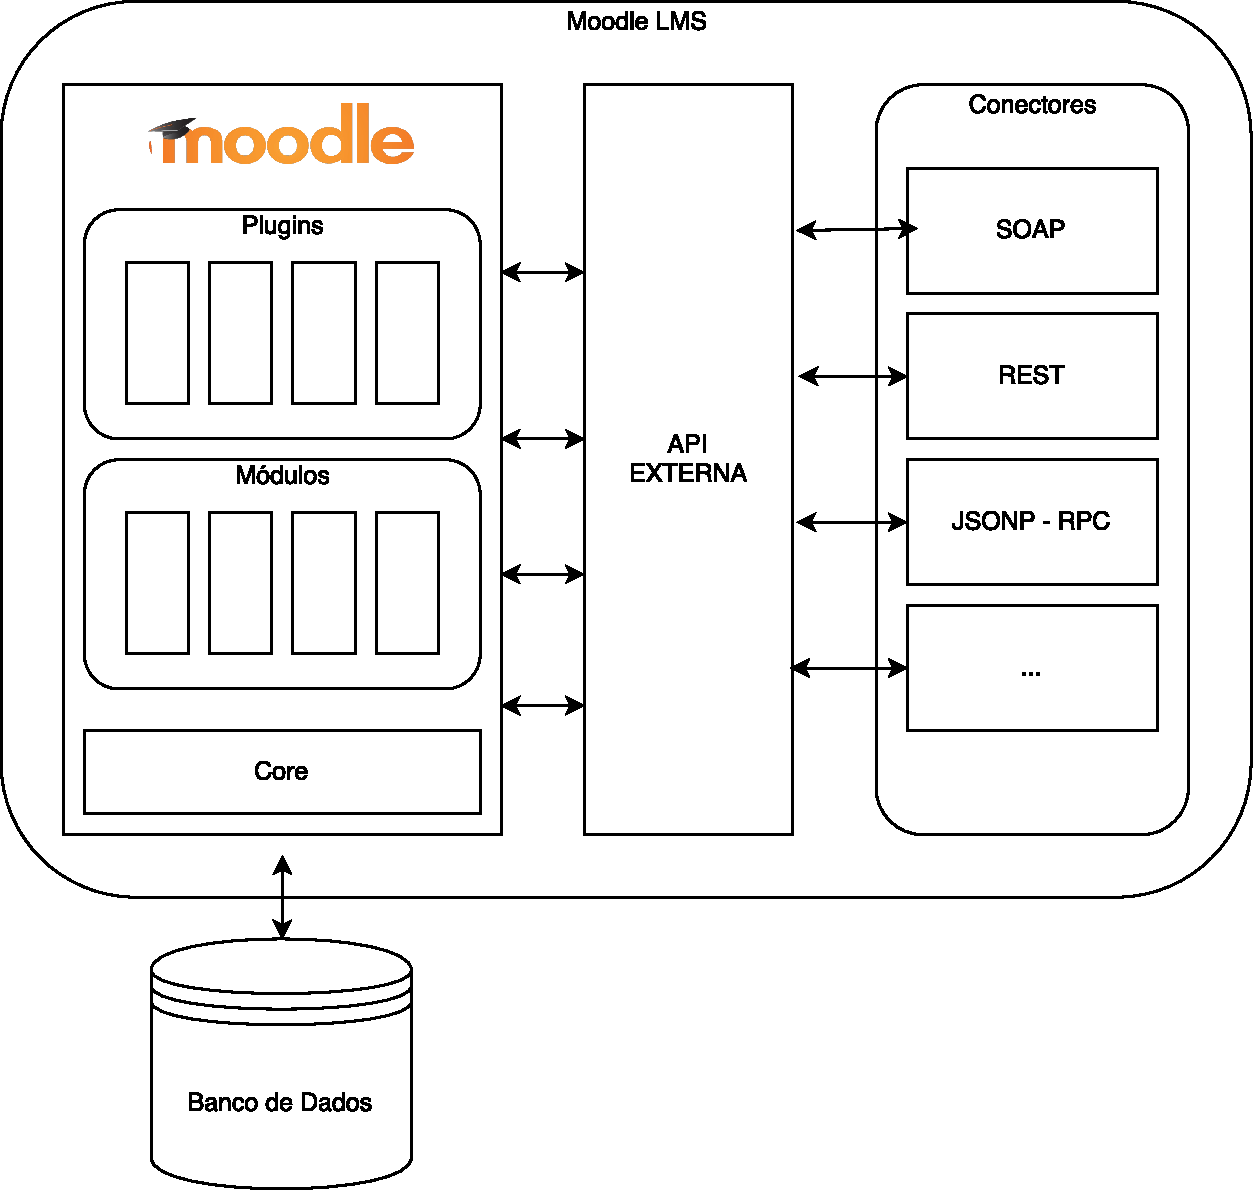
\includegraphics[scale=.65]{2_1.pdf}
    \caption{Arquitetura da camada de Serviços Moodle \cite{article:alier}}
    \label{moodle-arq}%
\end{figure}


